\chapter{Related Works}

Your related works, and your purpose and contribution which.
\section{Tasya Wiendhyra/1164086}
\subsection{binary classification dilengkapi ilustrasi gambar}
\begin{enumerate}
\item Binary classification yaitu berupa kelas positif dan kelas negatif. Klasifikasi biner adalah dikotomisasi yang diterapkan untuk tujuan praktis, dan dalam banyak masalah klasifikasi biner praktis, kedua kelompok tidak simetris - daripada akurasi keseluruhan, proporsi relatif dari berbagai jenis kesalahan yang menarik. Misalnya, dalam pengujian medis, false positive (mendeteksi penyakit ketika tidak ada) dianggap berbeda dari false negative (tidak mendeteksi penyakit ketika hadir).
\begin{figure}[ht]
\centering
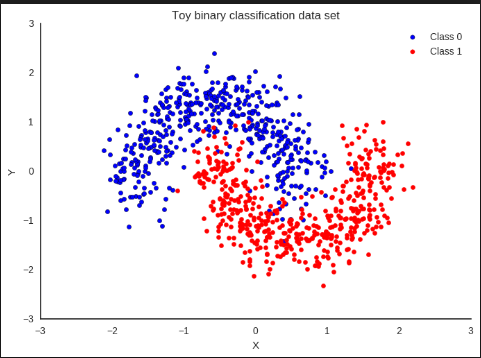
\includegraphics[scale=0.5]{figures/wiendh1.png}
\caption{Binary Classification}
\label{contoh}
\end{figure}
\end{enumerate}

\subsection{supervised learning dan unsupervised learning dan clustering dengan ilustrasi gambar}
\begin{enumerate}
\item Supervised learning adalah tugas pembelajaran mesin untuk mempelajari suatu fungsi yang memetakan input ke output berdasarkan contoh pasangan input-output. Ini menyimpulkan fungsi dari data pelatihan berlabel yang terdiri dari serangkaian contoh pelatihan. Dalam pembelajaran yang diawasi, setiap contoh adalah pasangan yang terdiri dari objek input (biasanya vektor) dan nilai output yang diinginkan (juga disebut sinyal pengawas). Algoritma pembelajaran yang diawasi menganalisis data pelatihan dan menghasilkan fungsi yang disimpulkan, yang dapat digunakan untuk memetakan contoh-contoh baru. Skenario optimal akan memungkinkan algoritma menentukan label kelas dengan benar untuk instance yang tidak terlihat. Ini membutuhkan algoritma pembelajaran untuk menggeneralisasi dari data pelatihan untuk situasi yang tidak terlihat dengan cara yang "masuk akal" (lihat bias induktif). Tugas paralel dalam psikologi manusia dan hewan sering disebut sebagai pembelajaran konsep. Contoh dibawah yaitu Supervised Learning dengan SVC.
\begin{figure}[ht]
\centering
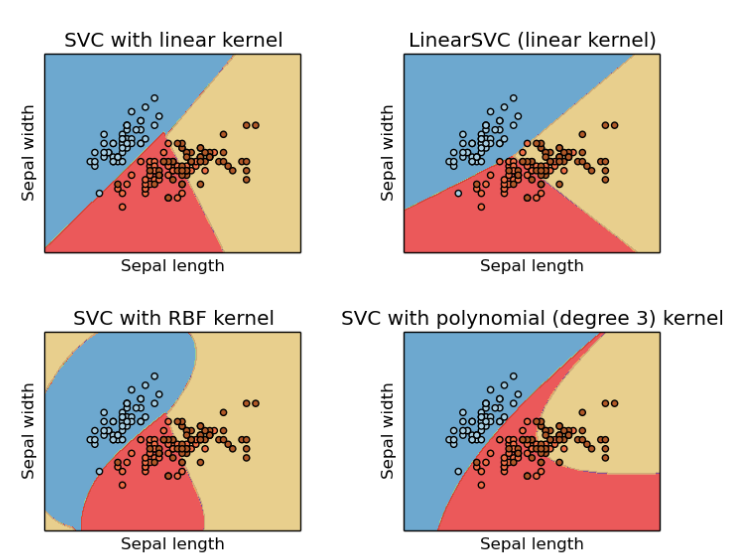
\includegraphics[scale=0.5]{figures/wiendh2.png}
\caption{Supervised Learning}
\label{contoh}
\end{figure}
\item Unsupervised learning adalah istilah yang digunakan untuk pembelajaran bahasa Ibrani, yang terkait dengan pembelajaran tanpa guru, juga dikenal sebagai organisasi mandiri dan metode pemodelan kepadatan probabilitas input. Analisis cluster sebagai cabang pembelajaran mesin yang mengelompokkan data yang belum diberi label, diklasifikasikan atau dikategorikan. Alih-alih menanggapi umpan balik, analisis klaster mengidentifikasi kesamaan dalam data dan bereaksi berdasarkan ada tidaknya kesamaan di setiap potongan data baru. BErikut merupakan contoh Unsupervised Learning dengan Gaussian mixture models.
\begin{figure}[ht]
\centering
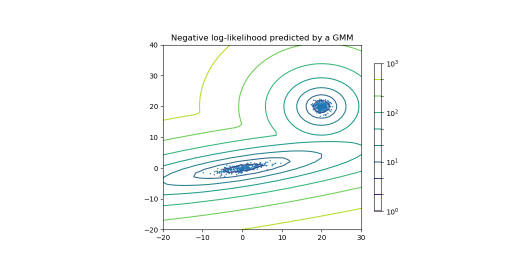
\includegraphics[scale=0.5]{figures/wiendh3.png}
\caption{Unsupervised Learning}
\label{contoh}
\end{figure}
\item Cluster analysis or clustering adalah tugas pengelompokan sekumpulan objek sedemikian rupa sehingga objek dalam kelompok yang sama (disebut klaster) lebih mirip (dalam beberapa hal) satu sama lain daripada pada kelompok lain (kluster). Ini adalah tugas utama penambangan data eksplorasi, dan teknik umum untuk analisis data statistik, yang digunakan di banyak bidang, termasuk pembelajaran mesin, pengenalan pola, analisis gambar, pengambilan informasi, bioinformatika, kompresi data, dan grafik komputer. Analisis Cluster sendiri bukan merupakan salah satu algoritma spesifik, tetapi tugas umum yang harus dipecahkan. Ini dapat dicapai dengan berbagai algoritma yang berbeda secara signifikan dalam pemahaman mereka tentang apa yang merupakan sebuah cluster dan bagaimana cara menemukannya secara efisien. Gagasan populer mengenai cluster termasuk kelompok dengan jarak kecil antara anggota cluster, area padat ruang data, interval atau distribusi statistik tertentu. Clustering karena itu dapat dirumuskan sebagai masalah optimasi multi-objektif. Algoritma pengelompokan dan pengaturan parameter yang sesuai (termasuk parameter seperti fungsi jarak yang akan digunakan, ambang kepadatan atau jumlah cluster yang diharapkan) tergantung pada set data individual dan penggunaan hasil yang dimaksudkan. Analisis kluster bukan merupakan tugas otomatis, tetapi proses berulang penemuan pengetahuan atau optimasi multi-objektif interaktif yang melibatkan percobaan dan kegagalan. Seringkali diperlukan untuk memodifikasi praproses data dan parameter model hingga hasilnya mencapai properti yang diinginkan.
\begin{figure}[ht]
\centering
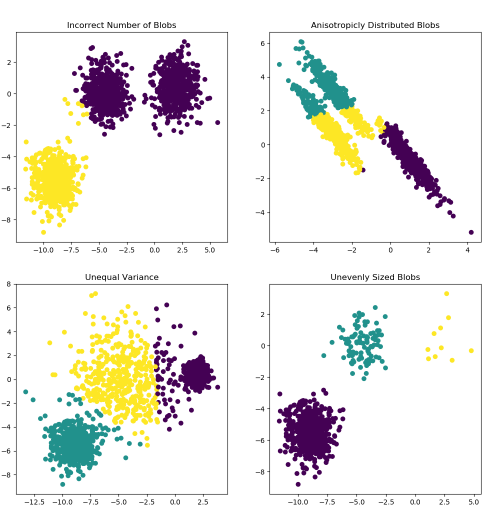
\includegraphics[scale=0.5]{figures/wiendh4.png}
\caption{Cluster}
\label{contoh}
\end{figure}
\end{enumerate}

\subsection{evaluasi dan akurasi dari buku dan disertai ilustrasi contoh
dengan gambar}
\begin{enumerate}
\item Evaluasi adalah tentang  bagaimana kita dapat mengevaluasi seberapa baik model bekerja dengan mengukur akurasinya. Dan akurasi akan didefinisikan sebagai persentase kasus yang diklasifikasikan dengan benar. Kita dapat menganalisis kesalahan yang dibuat oleh model, atau tingkat kebingungannya, menggunakan matriks kebingungan. Matriks kebingungan mengacu pada kebingungan dalam model, tetapi matriks kebingungan ini bisa menjadi sedikit sulit untuk dipahami ketika mereka menjadi sangat besar.
\begin{figure}[ht]
\centering
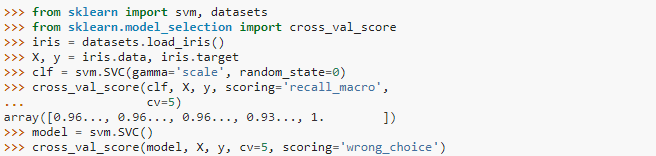
\includegraphics[scale=0.5]{figures/wiendh9.png}
\caption{ Evaluasi dan Akurasi}
\label{contoh}
\end{figure}
\end{enumerate}

\subsection{ bagaimana cara membuat dan membaca confusion matrix, buat confusion matrix }
\begin{enumerate}
\item Cara membuat dan membaca confusion matrix :
\begin{itemize}
\item 1)	Tentukan pokok permasalahan dan atributanya, misal gaji dan listik.
\item 2)	Buat pohon keputusan
\item 3)	Lalu data testingnya
\item 4)	Lalu mencari nilai a, b, c, dan d. Semisal a = 5, b = 1, c = 1, dan d = 3.
\item 5)	Selanjutnya mencari nilai recall, precision, accuracy, serta dan error rate.
\end{itemize}
\item Berikut adalah contoh dari confusion matrix :
\begin{itemize}
\item Recall =3/(1+3) = 0,75
\item Precision = 3/(1+3) = 0,75
\item Accuracy =(5+3)/(5+1+1+3) = 0,8
\item Error Rate =(1+1)/(5+1+1+3) = 0,2
\end{itemize}
\end{enumerate}

\subsection{bagaimana K-fold cross validation bekerja dengan gambar ilustrasi}
\begin{enumerate}
\item Cara kerja K-fold cross validation :
\begin{itemize}
\item 1)	Total instance dibagi menjadi N bagian.
\item 2)	Fold yang pertama adalah bagian pertama menjadi data uji (testing data) dan sisanya menjadi training data.
\item 3)	Lalu hitung akurasi berdasarkan porsi data tersebut dengan menggunakan persamaan.
\item 4)	Fold yang ke dua adalah bagian ke dua menjadi data uji (testing data) dan sisanya training data. 
\item 5)	Kemudian hitung akurasi berdasarkan porsi data tersebut.
\item 6)	Dan seterusnya hingga habis mencapai fold ke-K.
\item 7)	Terakhir hitung rata-rata akurasi K buah.
\end{itemize}
\begin{figure}[ht]
\centering
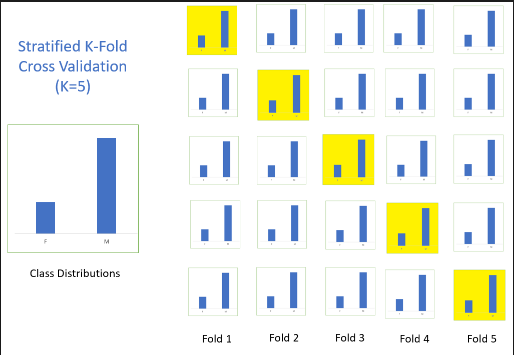
\includegraphics[scale=0.5]{figures/wiendh5.png}
\caption{K-fold cross validation }
\label{contoh}
\end{figure}
\end{enumerate}

\subsection{decision tree dengan gambar ilustrasi}
\begin{enumerate}
\item Decision Tree dalah metode pembelajaran yang diawasi non-parametrik yang digunakan untuk klasifikasi dan regresi. Tujuannya adalah untuk membuat model yang memprediksi nilai variabel target dengan mempelajari aturan keputusan sederhana yang disimpulkan dari fitur data.\\
Misalnya, dalam contoh di bawah ini, decision tree belajar dari data untuk memperkirakan kurva sinus dengan seperangkat aturan keputusan if-then-else. Semakin dalam pohon, semakin rumit aturan keputusan dan semakin bugar modelnya.
\begin{figure}[ht]
\centering
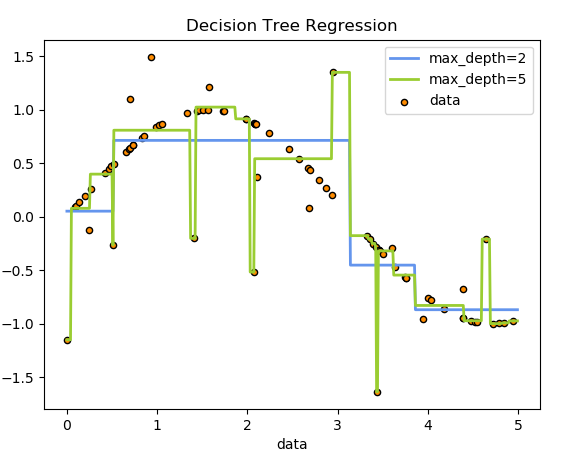
\includegraphics[scale=0.5]{figures/wiendh6.png}
\caption{Decision Tree}
\label{contoh}
\end{figure}
\end{enumerate}

\subsection{Information Gain dan entropi dengan gambar ilustrasi}
\begin{enumerate}
\item Information gain didasarkan pada penurunan entropi setelah dataset dibagi pada atribut. Membangun decision tree adalah semua tentang menemukan atribut yang mengembalikan perolehan informasi tertinggi (mis., Cabang yang paling homogen).
\begin{figure}[ht]
\centering
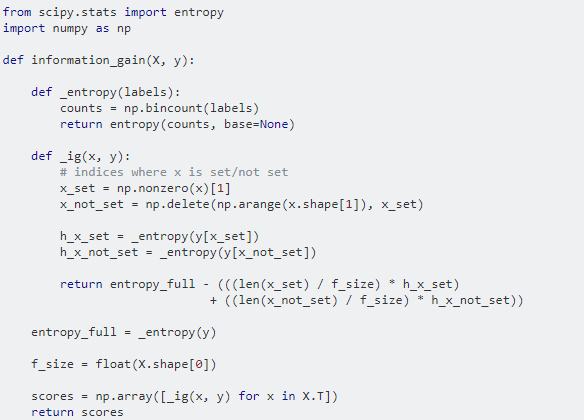
\includegraphics[scale=0.5]{figures/wiendh7.png}
\caption{Information gain}
\label{contoh}
\end{figure}
\item Entropi adalah ukuran keacakan dalam informasi yang sedang diproses. Semakin tinggi entropi, semakin sulit untuk menarik kesimpulan dari informasi itu. Membalik koin adalah contoh tindakan yang memberikan informasi yang acak. Untuk koin yang tidak memiliki afinitas untuk kepala atau ekor, hasil dari sejumlah lemparan sulit diprediksi. Mengapa? Karena tidak ada hubungan antara membalik dan hasilnya. Inilah inti dari entropi.
\begin{figure}[ht]
\centering
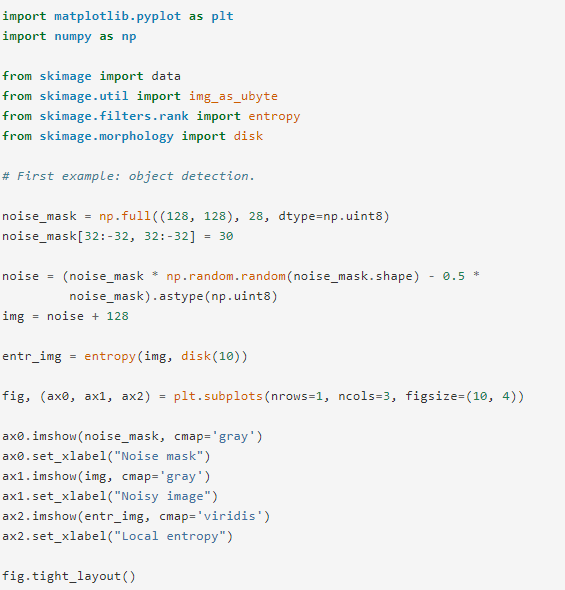
\includegraphics[scale=0.5]{figures/wiendh8.png}
\caption{Entropi}
\label{contoh}
\end{figure}
\end{enumerate}

\section{Annisa Fathoroni/1164067}
\subsection{Teori}
Penyelesaian Tugas Harian 3 ( No. 1-7 )
\begin{enumerate}
\item Binary Classification Dan Ilustrasi Gambarnya
\begin{itemize}
\item Pengertian Binary Classification / Klasifikasi Biner:

Klasifikasi biner atau binomial adalah tugas untuk mengklasifikasikan elemen-elemen dari himpunan tertentu ke dalam dua kelompok (memprediksi kelompok mana yang masing-masing dimiliki) berdasarkan aturan klasifikasi. Klasifikasi biner adalah dikotomisasi yang diterapkan untuk tujuan praktis, dan dalam banyak masalah klasifikasi biner praktis, kedua kelompok tidak simetris - daripada akurasi keseluruhan, proporsi relatif dari berbagai jenis kesalahan yang menarik. Misalnya, dalam pengujian medis, false positive (mendeteksi penyakit ketika tidak ada) dianggap berbeda dari false negative (tidak mendeteksi penyakit ketika hadir).

\item Ilustrasi Gambar Binary Classification:

\begin{figure}[ht]
\centering
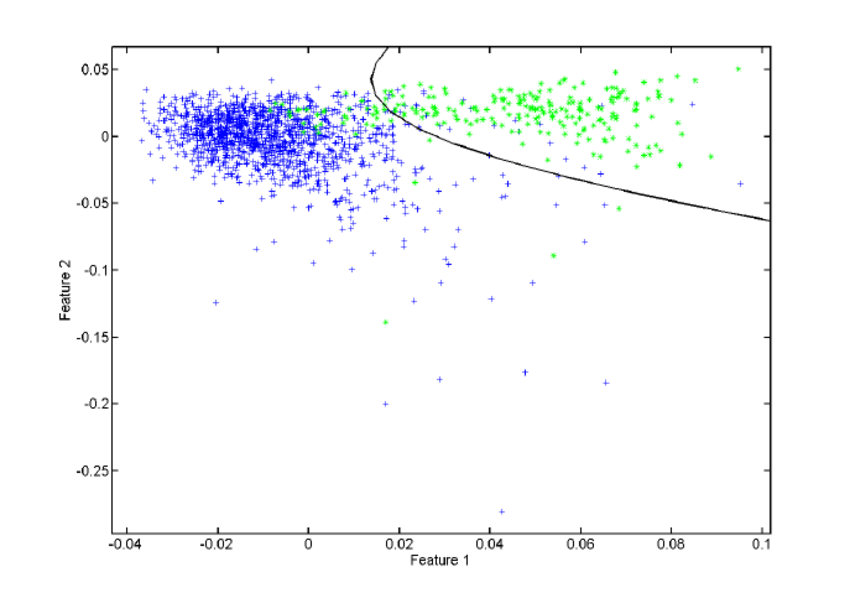
\includegraphics[scale=0.5]{figures/Chapter2-AnnisaFathoroni1.png}
\caption{capturing}
\label{contoh}
\end{figure}
\end{itemize}

\item Supervised Learning, Unsupervised Learning, Clustering Dan Ilustrasi Gambar
\begin{itemize}
\item Pengertian Supervised Learning dan Unsupervised Learning:

Supervised learning adalah sebuah pendekatan dimana sudah terdapat data yang dilatih, dan terdapat variable yang ditargetkan sehingga tujuan dari pendekatan ini adalah mengkelompokan suatu data ke data yang sudah ada, lain halnya dengan unsupervised learning, unsupervised learning tidak memiliki data latih, sehingga dari data yang ada, kita mengelompokan data tersebut menjadi 2 bagian atau 3 bagian dan seterusnya.

\begin{itemize}
\item Ilustrasi Gambar Supervised Learning dan Unsupervised Learning:

\begin{figure}[ht]
\centering
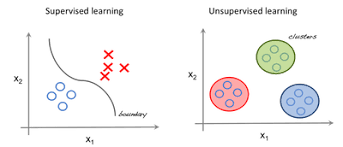
\includegraphics[scale=0.5]{figures/Chapter2-AnnisaFathoroni2.png}
\caption{capturing}
\label{contoh}
\end{figure}

\item Pengertian Clustering:

Clustering atau klasterisasi adalah metode pengelompokan data. Menurut Tan, 2006 clustering adalah sebuah proses untuk mengelompokan data ke dalam beberapa cluster atau kelompok sehingga data dalam satu cluster memiliki tingkat kemiripan yang maksimum dan data antar cluster memiliki kemiripan yang minimum. Clustering merupakan proses partisi satu set objek data ke dalam himpunan bagian yang disebut dengan cluster. Objek yang di dalam cluster memiliki kemiripan karakteristik antar satu sama lainnya dan berbeda dengan cluster yang lain. Partisi tidak dilakukan secara manual melainkan dengan suatu algoritma clustering. Oleh karena itu, clustering sangat berguna dan bisa menemukan group atau kelompokyang tidak dikenal dalam data. Clustering banyak digunakan dalam berbagai aplikasi seperti misalnya pada business inteligence, pengenalan pola citra, web search, bidang ilmu biologi, dan untuk keamanan (security). Di dalam business inteligence, clustering bisa mengatur banyak customer ke dalam banyaknya kelompok. Contohnya mengelompokan customer ke dalam beberapa cluster dengan kesamaan karakteristik yang kuat. Clustering juga dikenal sebagai data segmentasi karena clustering mempartisi banyak data set ke dalam banyak group berdasarkan kesamaannya. Selain itu clustering juga bisa sebagai outlier detection.

\begin{figure}[ht]
\centering
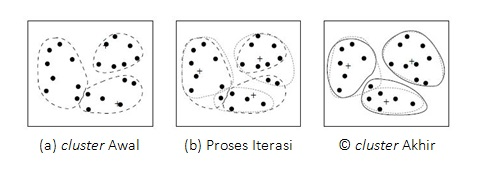
\includegraphics[scale=0.5]{figures/Chapter2-AnnisaFathoroni3.jpg}
\caption{capturing}
\label{contoh}
\end{figure}
\end{itemize}

\item Evaluasi, Akurasi Dan Ilustrasi Gambar

Evaluasi digunakan untuk memeriksa/memastikan dan mengevaluasi model dalam bekerja ( seberapa baik ) dengan mengukur keakuratannya. Kita juga dapat menanalisis kesalahan yang dibuat pada model yang dijalankan, tingkat kebingungan dan menggunakan matriks kebingunan. Accuracy akan didefinisikan sebagai presentasi kasus yang diklasifikasikan dengan benar. Accuracy lebih jelasnya adalah perbandingan kasus yang diidentifikasi benar dengan jumlah semua kasus.

\begin{figure}[ht]
\centering
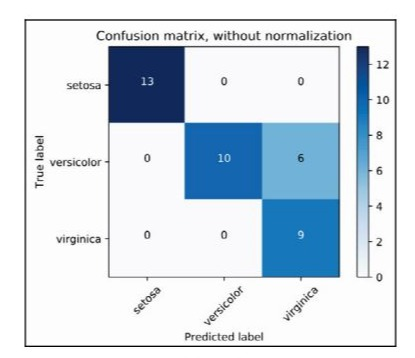
\includegraphics[scale=0.5]{figures/Chapter2-AnnisaFathoroni9.jpeg}
\caption{capturing}
\label{contoh}
\end{figure}

\begin{figure}[ht]
\centering
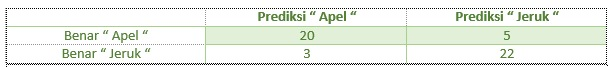
\includegraphics[scale=0.5]{figures/Chapter2-AnnisaFathoroni10.jpeg}
\caption{Akurasi}
\label{contoh}
\end{figure}

\item Cara membuat dan membaca confussion matrix:

Confusion matrix adalah suatu metode yang biasanya digunakan untuk melakukan perhitungan akurasi pada konsep data mining. Rumus ini melakukan perhitungan dengan 4 keluaran, yaitu: recall, precision, acuraccy dan error rate.
Rumus dari Error Rate = (b+c)/(a+b+c+d)
Keterangan:
jika hasil prediksi negatif dan data sebenarnya negatif.
jika hasil prediksi positif sedangkan nilai sebenarnya negatif.
jika hasil prediksi negatif sedangkan nilai sebenarnya positif.
jika hasil prediksi positif dan nilai sebenarnya positif.
Contoh perhitungan confusion matrix adalah sebagai berikut, yaitu pengambilan keputusan untuk mendapatkan bantuan beasiswa. Saya menggunakan dua atribut, yaitu rekening listrik dan gaji. Ini adalah pohon keputusannya:
yang pertama kita lakukan yaitu mencari 4 nilai yaitu a,b,c, dan d:
a= 5
b= 1
c= 1
d= 3
Kemudian kita dapat mencari nilai Recall, Precision, accuracy dan Error Rate:
Recall =3/(1+3) = 0,75
Precision = 3/(1+3) = 0,75
Accuracy =(5+3)/(5+1+1+3) = 0,8
Error Rate =(1+1)/(5+1+1+3) = 0,2

\begin{figure}[ht]
\centering
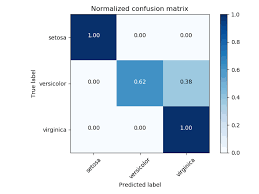
\includegraphics[scale=0.5]{figures/Chapter2-AnnisaFathoroni4.png}
\caption{capturing}
\label{contoh}
\end{figure}

\item Cara Bekerja K-Fold Cross Validation:

Total instance dibagi menjadi N bagian. 
Fold ke-1 adalah ketika bagian ke-1 menjadi data uji (testing data) dan 
Sisanya menjadi data latih (training data). Selanjutnya, hitung akurasi berdasarkan porsi data tersebut. Perhitungan akurasi tersebut dengan menggunakan persamaan sebagai berikut: 
Fold ke-2 adalah ketika bagian ke-2 menjadi data uji (testing data) dan sisanya menjadi data latih (training data). Selanjutnya, hitung akurasi berdasarkan porsi data tersebut.  
Demikian seterusnya hingga mencapai fold ke-K. Hitung rata-rata akurasi dari K buah akurasi di atas. Rata-rata akurasi ini menjadi akurasi final.

\begin{figure}[ht]
\centering
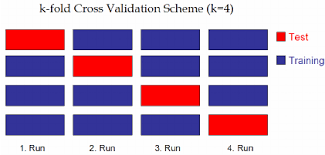
\includegraphics[scale=0.5]{figures/Chapter2-AnnisaFathoroni5.png}
\caption{capturing}
\label{contoh}
\end{figure}

\item Decision Tree

Decision tree adalah salah satu metode klasifikasi yang paling populer karena mudah diinterpretasikan oleh manusia. Decision tree digunakan untuk pengenalan pola dan termasuk dalam pengenalan pola secara statistik.

\begin{figure}[ht]
\centering
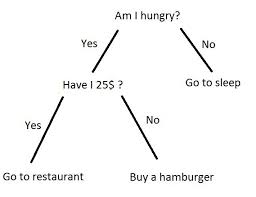
\includegraphics[scale=0.5]{figures/Chapter2-AnnisaFathoroni6.jpg}
\caption{capturing}
\label{contoh}
\end{figure}

\item Information Gain dan Entropi

Information gain adalah salah satu atribute selection measure yang digunakan untuk memilih test atribute tiap node pada tree. Atribut dengan information gain tertinggi dipilih sebagai test atribut dari suatu node. Ada 2 kasus berbeda pada saat penghitungan Information Gain, pertama untuk kasus penghitungan atribut tanpa missing value dan kedua, penghitungan atribut dengan missing value.

\begin{figure}[ht]
\centering
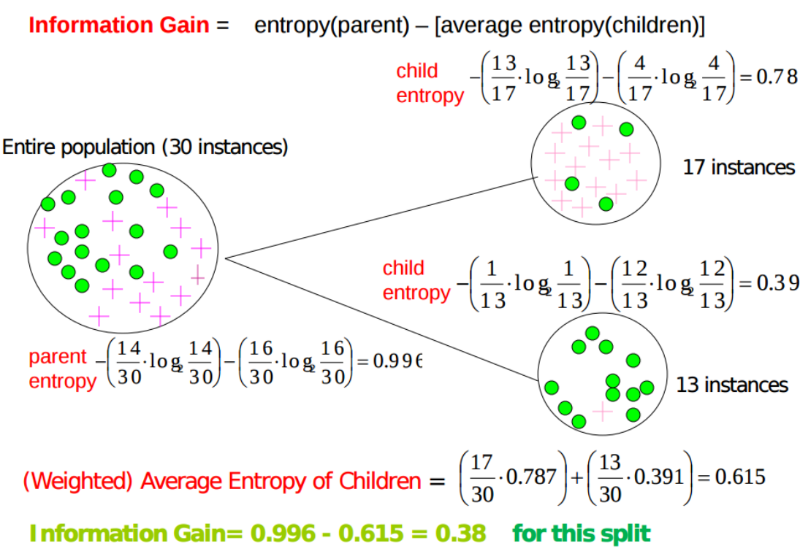
\includegraphics[scale=0.5]{figures/Chapter2-AnnisaFathoroni7.png}
\caption{capturing}
\label{contoh}
\end{figure}

Entropi adalah suatu parameter untuk mengukur tingkat keberagaman (heterogenitas) dari kumpulan data. Semakin heterogen, nilai entropi semakin besar. 
\begin{figure}[ht]
\centering
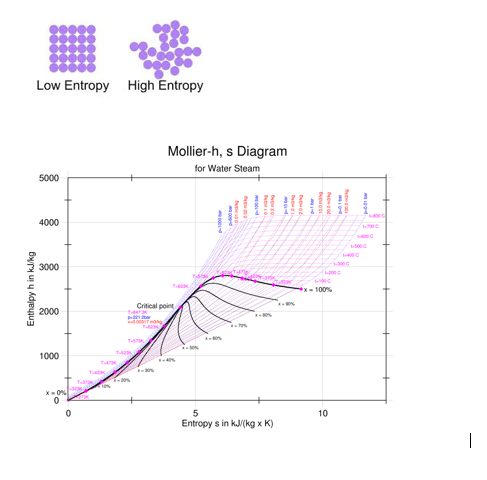
\includegraphics[scale=0.5]{figures/Chapter2-AnnisaFathoroni8.png}
\caption{capturing}
\label{contoh}
\end{figure}

\end{itemize}
\end{enumerate}